\subsection*{Groep IO}

\subsubsection*{Deze week}
\begin{itemize}
\item Model van een ebike gemaakt (zie figuur \ref{img:fiets}).
\item Animatie toegevoegd zodat de ebike binnen komt rijden in het oplaadstation.
\item Mac OSX ge\"installeerd in een virtualbox om xcode te kunnen gebruiken om de app te maken.
\item Stuk thesis geschreven.
\item modelviewer ge\"update op de solarpowerdbikes site.
\item modelviewer ge\"update op de mediawebsite + station kan weer draaien met de muis.
\item gewerkt aan PHP sessions om de app te beveiligen tegen kwaadwillenden.
\item onderscheid gemaakt tussen admin en user login, deze komen na in te loggen op een andere pagina terecht.
\item CSS animaties gemaakt voor de reserveerpagina.
\item een begin gemaakt aan het herschrijven van URLs zodat niet achter iedere pagina .php of .html geschreven hoeft te worden.

\end{itemize}

\noindent Het nieuwe CSS design van de applogin en appreserveren pagina zijn te vinden op:\\ \url{http://solarpoweredbikes.tudelft.nl/eud/app_login}\\

\noindent Username: sunrise\\
\noindent Password: helemaalmooi\\

\noindent De media website is via de volgende link te bekijken:\\
\url{http://solarpoweredbikes.tudelft.nl/media/index.html}\\

\noindent Met de WASD en pijltjestoetsen kun je in de 'debug' modus rondlopen.

\subsubsection*{Volgende weken}
\begin{itemize}
\item Verder met de Thesis
\item HTTPS beveiliging
\item Android en iPhone app
\item PHP sessions bugvrij maken
\item mediawebsite invullen met informatie
\item gegevens uit de database mooi kunnen weergeven met CSS en WebGL
\end{itemize}


\begin{figure}[!h]
\begin{center}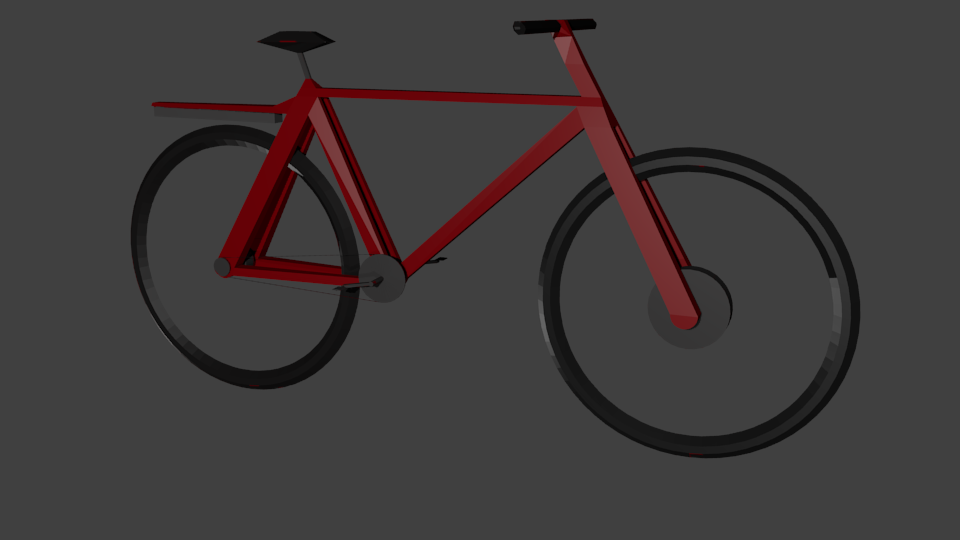
\includegraphics[width=12cm]{ebike.png}
\caption{Render van het ebike model}
\label{img:fiets}
\end{center}
\end{figure}
